\documentclass[11pt]{book}
\usepackage[left=1in,right=1in,bottom=1in,top=1in]{geometry}
\usepackage{graphicx}  		 % allows use of graphic figures
\usepackage{varioref}  		 % smart page, figure, table, and equation referencing
\usepackage{wrapfig}   		 % wrap figures/tables in text (i.e., Di Vinci style)
\usepackage{threeparttable}  % tables with footnotes
\usepackage{subfigure} 		 % allows multiple figures treated as one
\usepackage{subfigmat}  	 % matrices of similar subfigures, aka small mulitples
\usepackage{wrapfig}
\usepackage{amsmath}  		 % loads extra math symbols
\usepackage{amssymb}  		 % also loads amsfonts
\usepackage{empheq}
\usepackage{mathrsfs}
\usepackage{hyperref}
\hypersetup{linkcolor=blue,colorlinks=true,urlcolor=blue}
\usepackage{enumitem}
\usepackage[toc,page]{appendix}

\usepackage{url}             % handle URLs, directories, e-mail addresses
\usepackage{cite}            % make sequential citations look nice
\usepackage{listings}        % for pretty printing of program code
\usepackage{xcolor}
\usepackage{soul}            % defines underlining with line breaks for abstract
\usepackage{dcolumn}
 \newcolumntype{d}{D{.}{.}{-1}}
\usepackage{booktabs}
\usepackage{pdflscape}
\usepackage{tikz}
\usetikzlibrary{arrows,shapes,positioning,shadows,trees}


\definecolor{gray}{rgb}{0.4,0.4,0.4}
\definecolor{darkblue}{rgb}{0.0,0.0,0.6}
\definecolor{cyan}{rgb}{0.0,0.6,0.6}
\definecolor{maroon}{rgb}{0.5,0.0,0.0}
\definecolor{darkgreen}{rgb}{0.0,0.5,0.0}


\newcommand{\degree}{$^{\circ}$}
\newcommand{\inltt}[1]{\tikz[anchor=base,baseline]\node[inner sep=3pt,
rounded corners,outer sep=0,draw=black!30,fill=black!05]{\small\texttt{#1}};}
\newcommand{\inlsh}[1]{\tikz[anchor=base,baseline]\node[inner sep=2pt,
outer sep=0,fill=black!05]{\texttt{#1}};}

\makeatletter\@addtoreset{chapter}{part}\makeatother%
\makeatletter\@openrightfalse

%%% PRETTY TITLE PAGE FOR PDF DOC
%%%-----------------------------------------------------------------------------

\makeatletter
\newlength\drop
\newcommand{\br}{\hfill\break}
\newcommand*{\prettytitle}{%
    \thispagestyle{empty}
    \begingroup
    \drop = 0.1\textheight
    \vspace*{\baselineskip}
    \vfill
    \hbox{%
      \hspace*{0.1\textwidth}%
      \rule{1pt}{\dimexpr\textheight-28pt\relax}%
      \hspace*{0.05\textwidth}% 
      \parbox[b]{0.85\textwidth}{%
        \vbox{%
          %{\includegraphics[width=0.33\textwidth]{images/}\par}
          \vskip1.00\baselineskip
          {\Huge\bfseries\raggedright\@title\par}
          \vskip1\baselineskip
          {\huge\bfseries Version 1.0 \par}
          \vskip4\baselineskip
          {\huge\bfseries \textcolor{darkgreen}{Developer's Guide}\par}
          \vskip1.0\baselineskip
          {\large\bfseries\@date\par}
          \vspace{0.3\textheight}
          {\small\noindent\@author}\\[\baselineskip]
        }% end of vbox
      }% end of parbox
    }% end of hbox
    \vfill
    \null
\endgroup}
%%%-----------------------------------------------------------------------------


\title{HPC AMR Software Framework}
\date{\today}

\author{Andrew Kirby, Ph.D.}

\begin{document}
\prettytitle

\section*{Document Summary}
This document presents an overview of the HPC AMR framework which is designed to provide an infrastructure for arbitrary physics and solvers on structured and unstructured grids with 
adaptive mesh refinement (AMR). An implementation procedure is outlined for new solvers and physics kernels.

\tableofcontents

\part{Theory and Background}
\chapter{Computational Grids}
Commonly in Computer-aided engineering (CAE), the use of a mesh or grid is used to tessellate and discretize a computational geometric domain. 
The grid can be classified into two categories for our purposes: structured and unstructured. 
Structured grids are composed of elements which are the same size and orientation throughout the computational domain. 
The simplest example of a structured grid is a Cartesian grid as shown in Fig.~(\ref{grid-types})(a) where the side lengths 
of an element are equal and the outward normal vectors align with the Cartesian unit vectors, e.g. $\hat{n} = (1,0,0)$. 
Alternative to structured grids, unstructured meshes allow for arbitrary element size and shape with irregular connectivity 
as shown in Fig.~(\ref{grid-types})(b). 

\begin{figure}[h]
 \begin{subfigmatrix}{2}% number of columns
  \subfigure[Structured Grid]{
\includegraphics{Images/structured-grid-2.png}}
  \subfigure[Unstructured Grid]{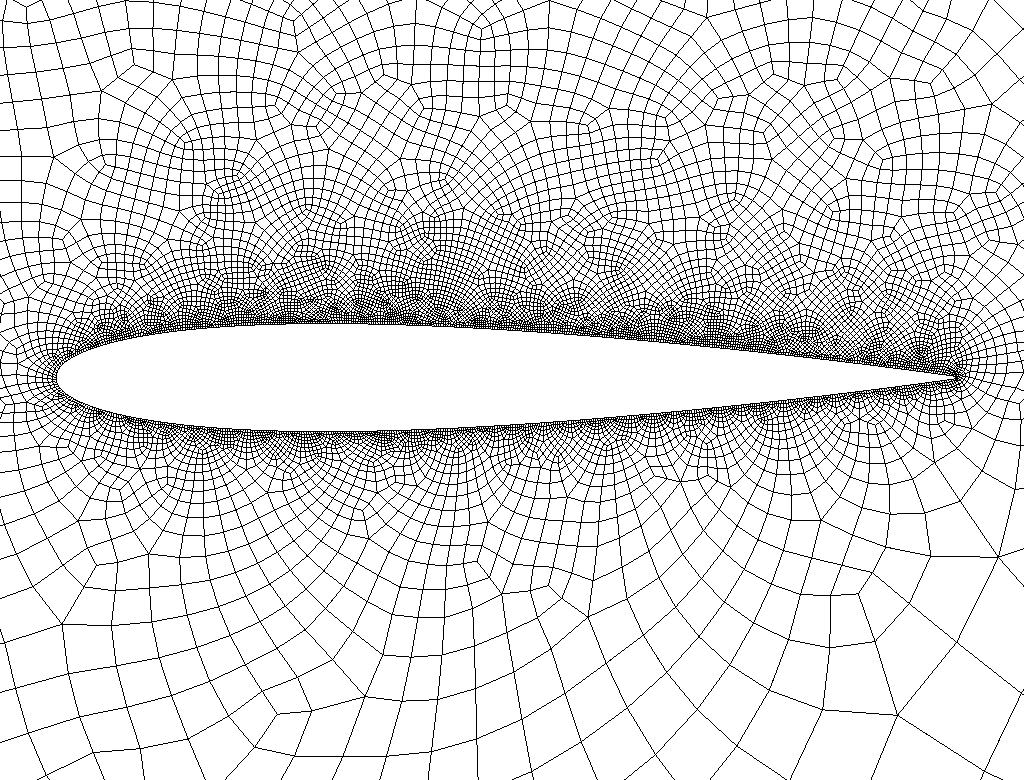
\includegraphics{Images/unstructured-grid.png}}
 \end{subfigmatrix}
 \caption{Computational Grids}
 \label{grid-types}
\end{figure}

Structured grids contain regularly-shaped elements allowing for ease of software implementation and regularity in element shapes.
This can lead to high computational efficiency.
However, simulation of complex geometries is non-trivial since the grid does not conform to bodies. 
There are several techniques to approximate complex geometries such as cut-cell methods and immersed boundary methods.
\medskip

Unstructured grids, on the other hand, allow for complex non-trivial geometries to be discretized very accurately. 
However, implementation of unstructured solvers is much more difficult and can be less computationally efficient.

\newpage
\section{Adaptive Mesh Refinement (AMR)}
Adaptive mesh refinement (AMR) is the procedure of modifying the computational mesh to more accurately capture physics features.
This modification procedure generally adds grid resolution into regions of physics features by various grid adaption strategies.
The grid adaption strategies can be classified into three categories: \textit{r}-refinement, \textit{h}-refinement, and \textit{p}-refinement.
\bigskip

\noindent
\underline{\textbf{\textit{r}-refinement}}:\\
\textit{r}-refinement is the procedure of modifying the mesh resolution by moving the mesh nodes but not changing the number of mesh nodes. 
Fig.~(\ref{grid-refinement})(a) demonstrates \textit{r}-refinement by moving mesh nodes to the curved region of the geometry without modifying 
the number of grid elements
\bigskip

\noindent
\underline{\textbf{\textit{h}-refinement}}:\\
\textit{h}-refinement is the procedure of modifying the mesh resolution by adding mesh nodes through grid element subdivision.
Fig.~(\ref{grid-refinement})(b) demonstrates \textit{h}-refinement of quad and triangle elements. This type of mesh adaption 
can lead to non-conforming elements with \textit{hanging} nodes as seen in Fig.~(\ref{grid-refinement})(d) indicated by the red node.
\bigskip

\noindent
\underline{\textbf{\textit{p}-refinement}}:\\
\textit{p}-refinement is the procedure of enhancing the order of solution accuracy inside the element.
This is common in Finite Element Methods in which the polynomial degree of the solution expansion is increased.
Fig.~(\ref{grid-refinement})(c) demonstrates \textit{p}-refinement where the original solution is approximated 
by linear functions then enhanced by using quadratic functions to approximate the solution.


\begin{figure}[h]
 \begin{subfigmatrix}{2}% number of columns
  \subfigure[\textit{r}-refinement]{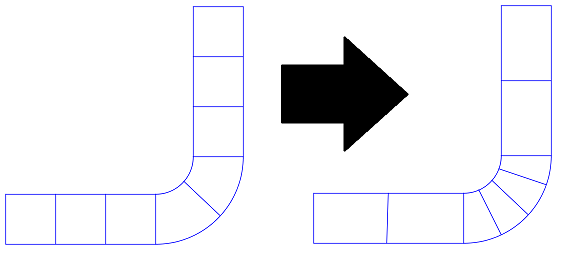
\includegraphics{Images/Mesh-R-Refinement.png}}
  \subfigure[\textit{h}-refinement]{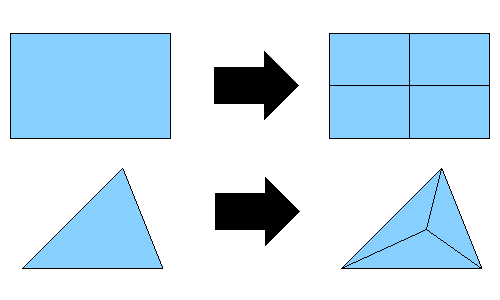
\includegraphics{Images/Mesh-H-Refinement.png}}
  \subfigure[\textit{p}-refinement]{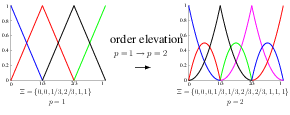
\includegraphics{Images/P-Refinement.png}}
  \subfigure[hanging nodes]{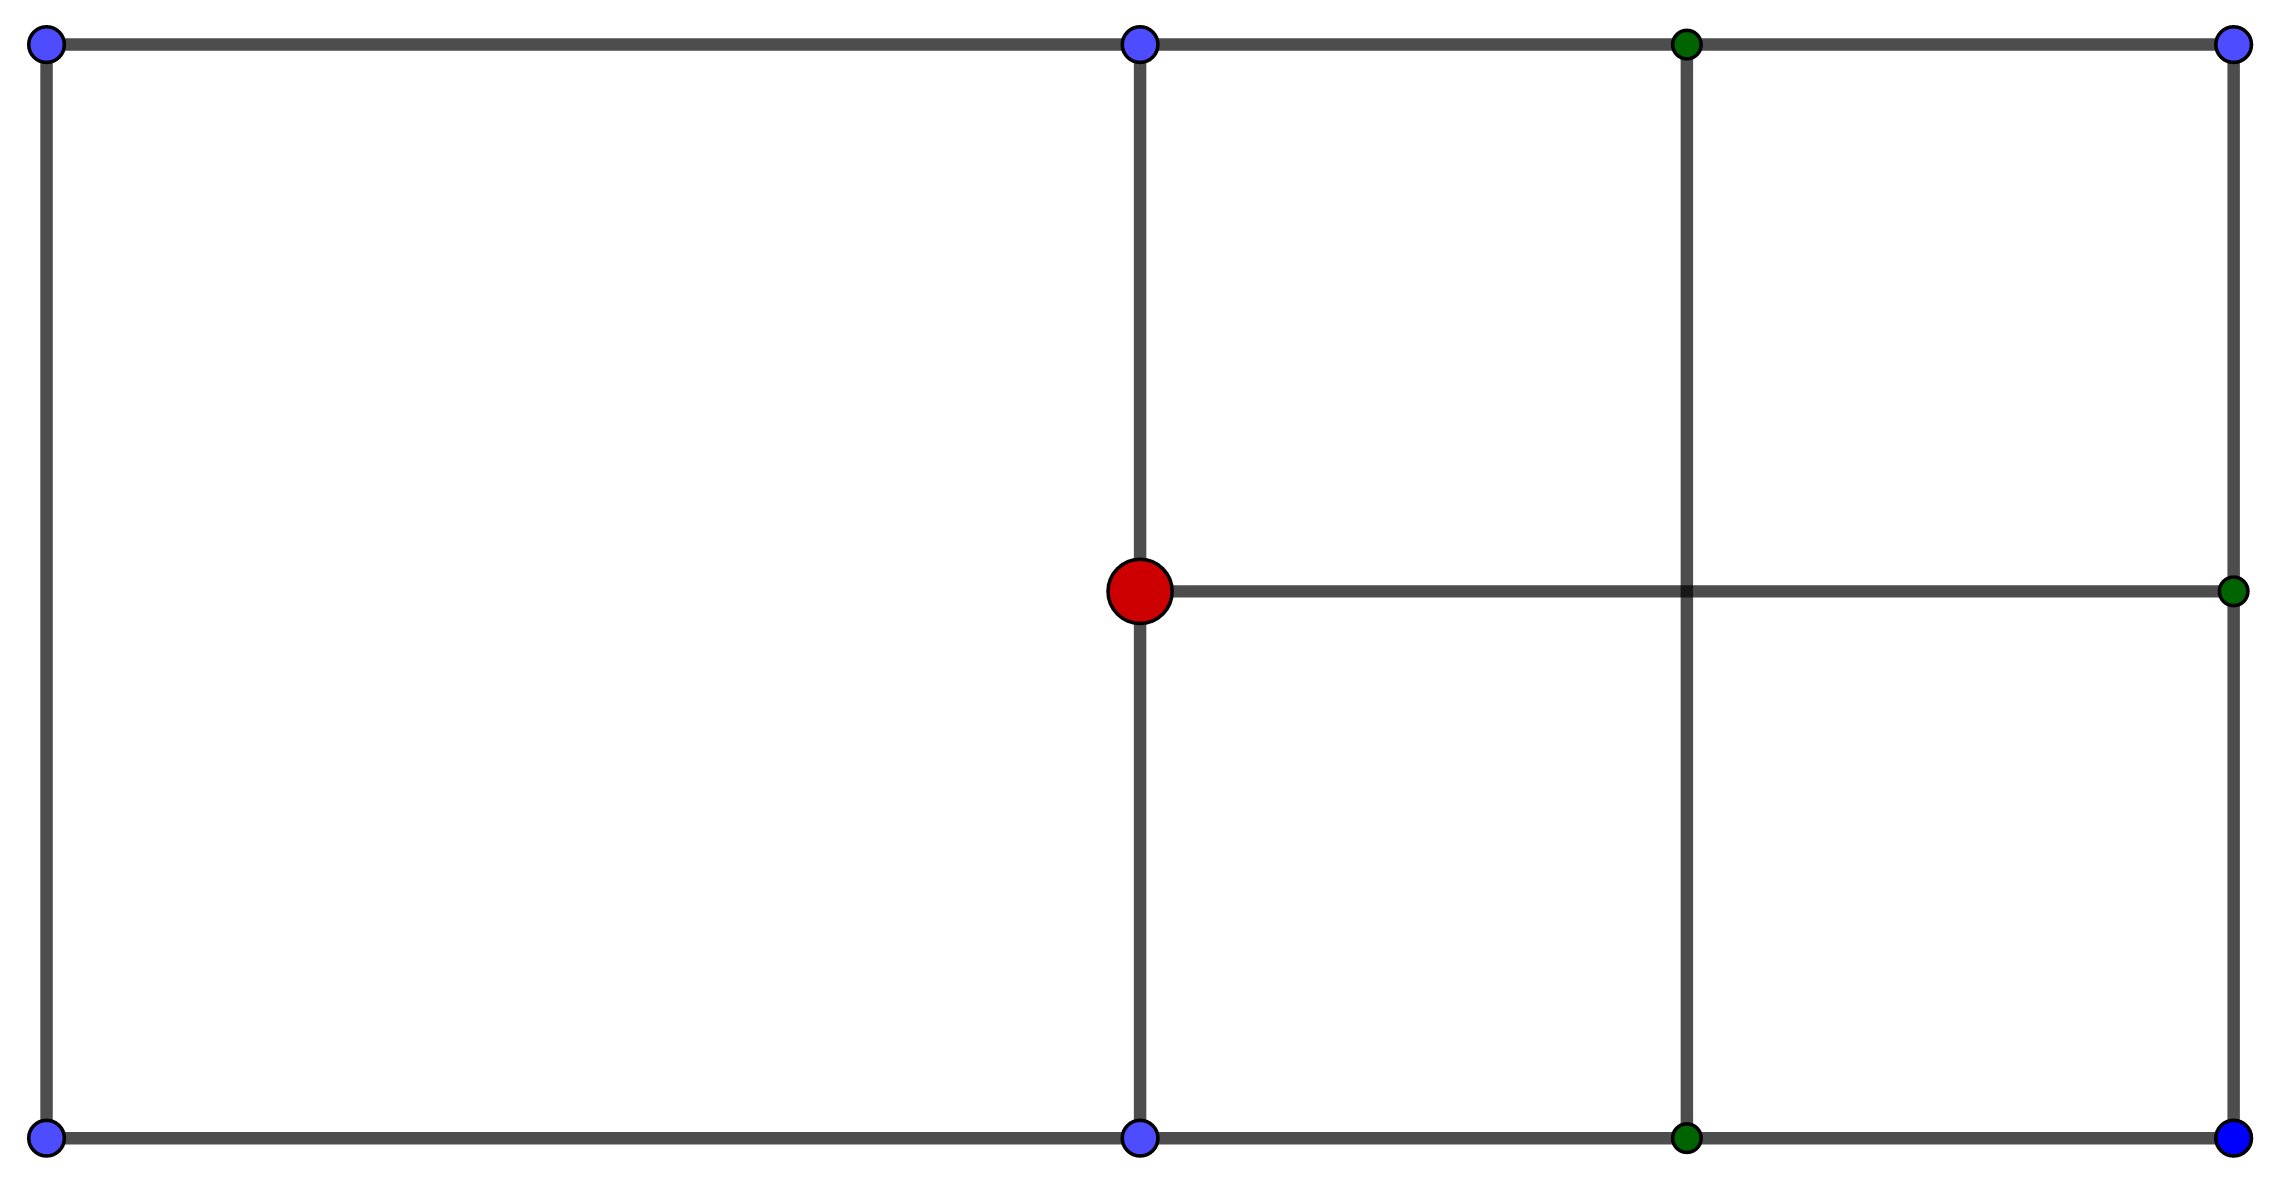
\includegraphics{Images/hanging-node.png}}
 \end{subfigmatrix}
 \caption{Grid Adaption Strategies}
 \label{grid-refinement}
\end{figure}





\subsection{AMR Data Structured Philosophies: Patches and Octrees}
Adaptive mesh refinement frameworks typically implement data structures into two classes: patch-based and octree-based.
In patch-based AMR, the computational mesh is decomposed into a collection of logically rectangular overlapping 
patches that form mesh levels, each of fixed spatial resolution, as shown in Fig.~(\ref{AMR-data-structures})(a). 
The spatial resolution ratio between two consecutive mesh levels, known as the refinement ratio, is generally two, 
although other refinement ratios are possible. The computational mesh structure starts at the coarsest level which 
tessellates the entire computational domain using the coarsest spatial resolution prescribed by the user. 
Finer mesh levels are constructed sequentially, from coarsest to finest, by tagging cells for refinement, 
clustering them into patches, and refining the solution. These newly refined patches overlap coarser level patches 
which require their element solutions to be filled using the finer level solution. 
In addition to requiring their solutions overwritten, non-overlapped coarse elements touching a 
coarse-fine element boundary require a corrected flux from the fine level to maintain conservation. 
If conservation is not maintained, numerical issues may arise.
\medskip

In contrast to patch-based AMR methods where blocks are permitted to overlap, octree-based AMR methods make use of recursive encoding algorithms 
for non-overlapping mesh refinement. Thus, there is no need to fill covered coarse level solutions since octree-based AMR methods do not contain 
overlapping mesh elements as shown in Fig.~(\ref{AMR-data-structures})(b). 
However, suppose an algorithm requires overlapping coarse mesh elements such as geometric multigrid, surrogate meshes can be used to contain the 
storage of the overlapped coarse elements. In addition, each octree-mesh element may contain a patch of data. 
Therefore octree-based data structures can possess the same capabilities as patch-based data structures but allow for increased implementation flexibility. 

\begin{figure}[t]
 \begin{subfigmatrix}{2}% number of columns
  \subfigure[Patch-based AMR]{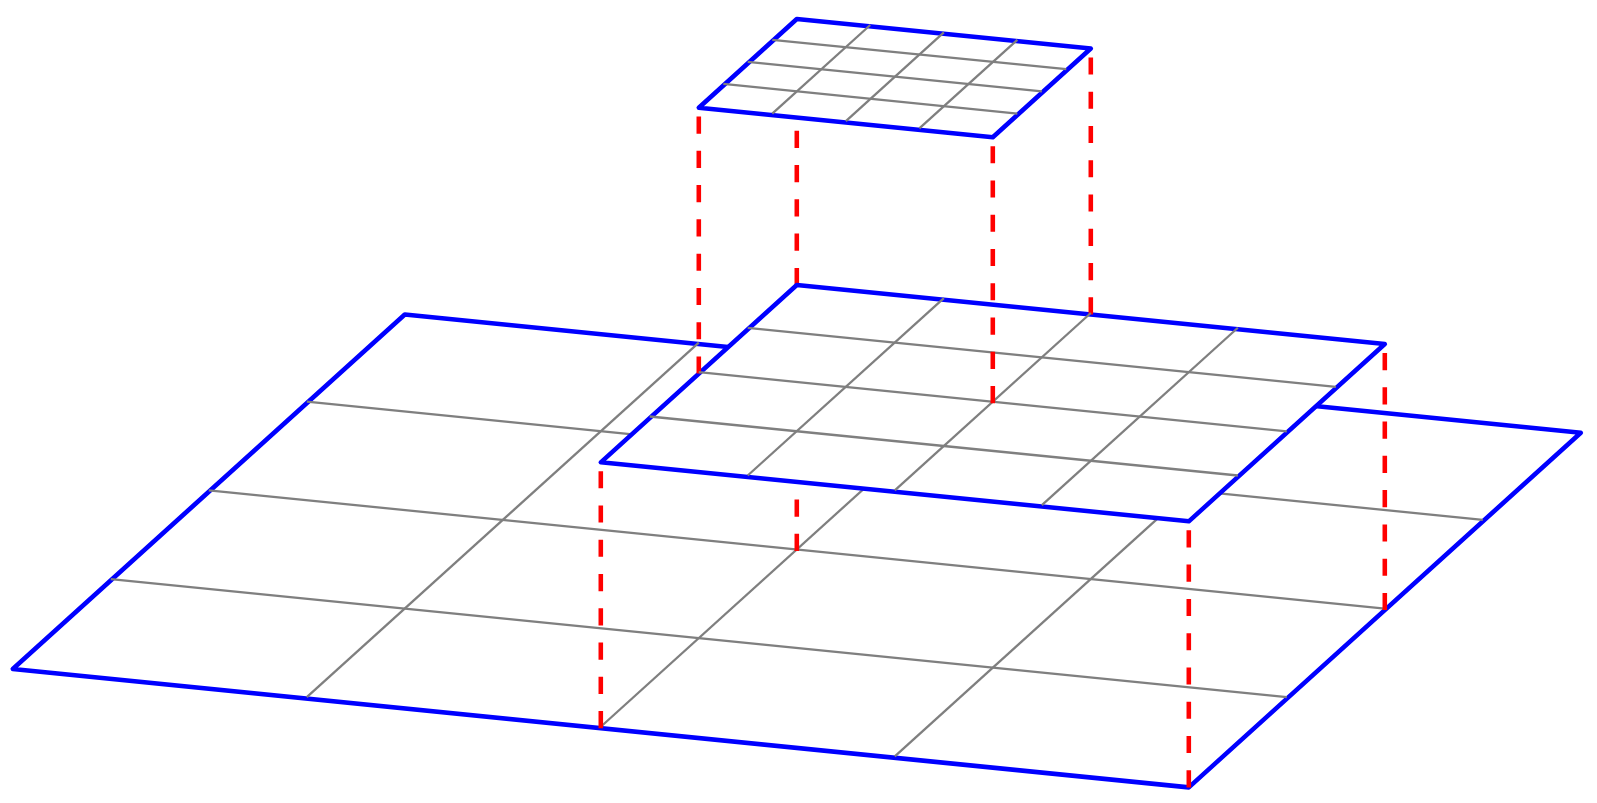
\includegraphics{Images/AMR/patch-based-amr.png}}
  \label{Patch-AMR}
  \subfigure[Octree-based AMR]{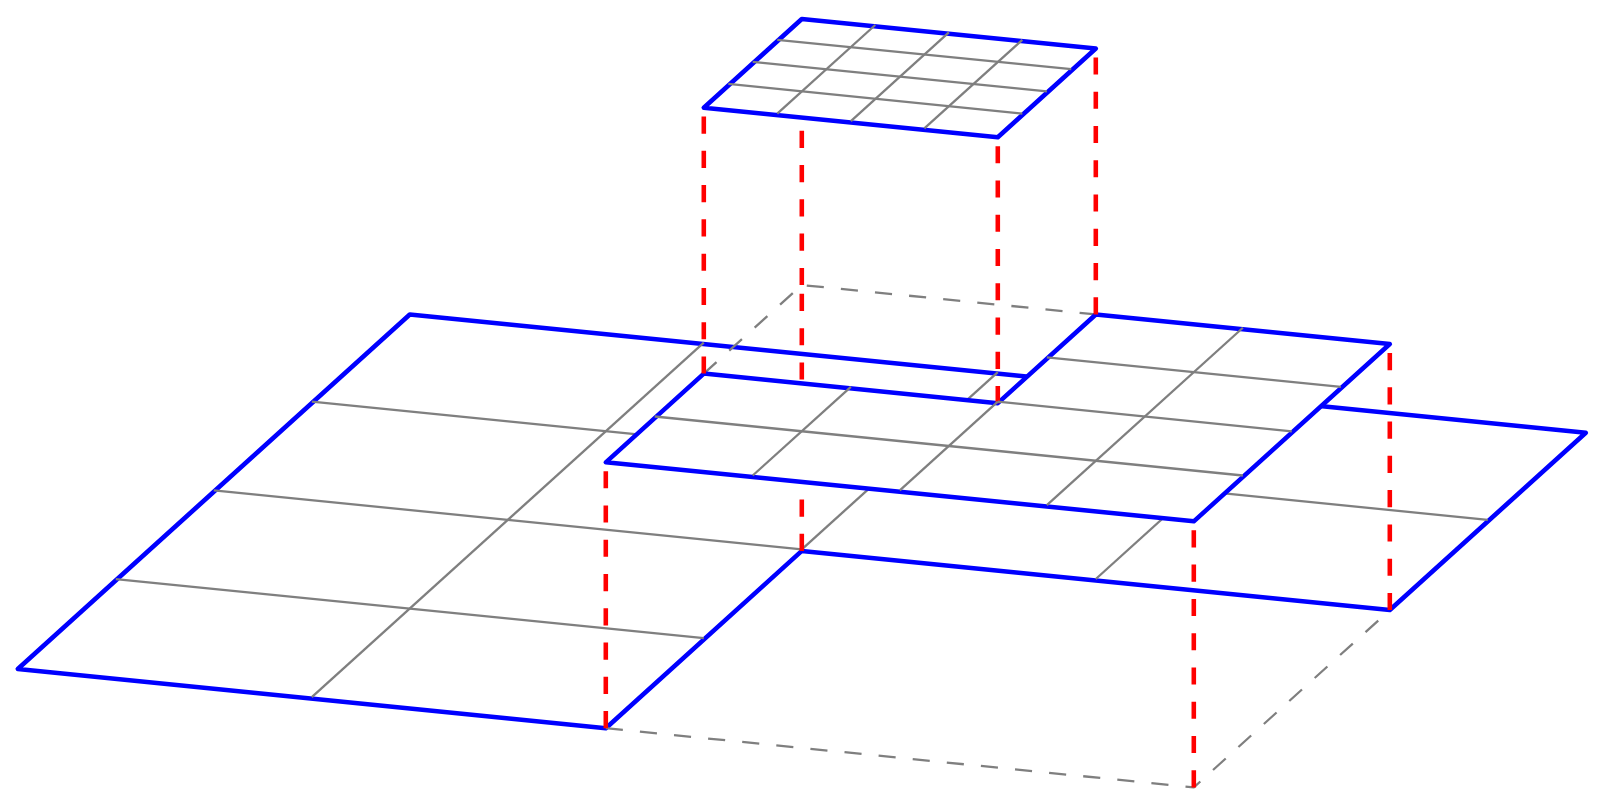
\includegraphics{Images/AMR/octree-amr.png}}
  \label{Octree-AMR}
 \end{subfigmatrix}
 \caption{Patch-based AMR frameworks contain mesh elements that are overlapped by finer level mesh elements in contrast to octree-based AMR methods which do not contain overlapped mesh elements.}
 \label{AMR-data-structures}
\end{figure}


\newpage
\subsection{Comparison of Parallel Communication Protocols}
Octree-based AMR frameworks traditionally implement the parallel communication pattern by doing a direct exchange of data 
required by the computational stencil with multiple fringe layers as necessary. When parallel communication is invoked, 
the elements on a grid-partition boundary are communicated to the respective neighboring processor by packing and sending 
a copy of its solution data. This can be viewed as a direct solution exchange at the grid-partition boundary.
\medskip

In contrast, patch-based AMR frameworks typically implement parallel communication 
patterns composed of data transfers between mesh level interfaces. 
These data communication transfers first occur in a coarse-to-fine level procedure, 
which requires a refinement operator. In the solution process, the solver is executed for 
one computational time step on each mesh level, then the solution on the fine level 
is transferred down to the coarser levels via a coarsen operator. Fig.~(\ref{Patch-AMR-Solve}) 
demonstrates the patch-based AMR communication and flow solve execution pattern.
\medskip

Additionally, a flux correction is required for conservation as the flux calculated 
on the fine level is different from the flux calculated on the coarse level. 
Thus, additional communication of the flux calculated on the fine level to the 
coarse level is required, which is used to correct the coarse level solution. 
Further, the coarsen operator adds extraneous computations at every computational 
time step. Many of the patch-based AMR frameworks are implemented using this communication 
protocol, which can be difficult for finite-element method implementation. 
If the parallel communication pattern of direct solution is used, patch-based AMR 
would be perfectly acceptable for use and ease of development for finite-element methods.
\bigskip

\begin{figure}[t]
 \begin{subfigmatrix}{3}% number of columns
  \subfigure[coarse-to-fine level communication via refinement operator]
  {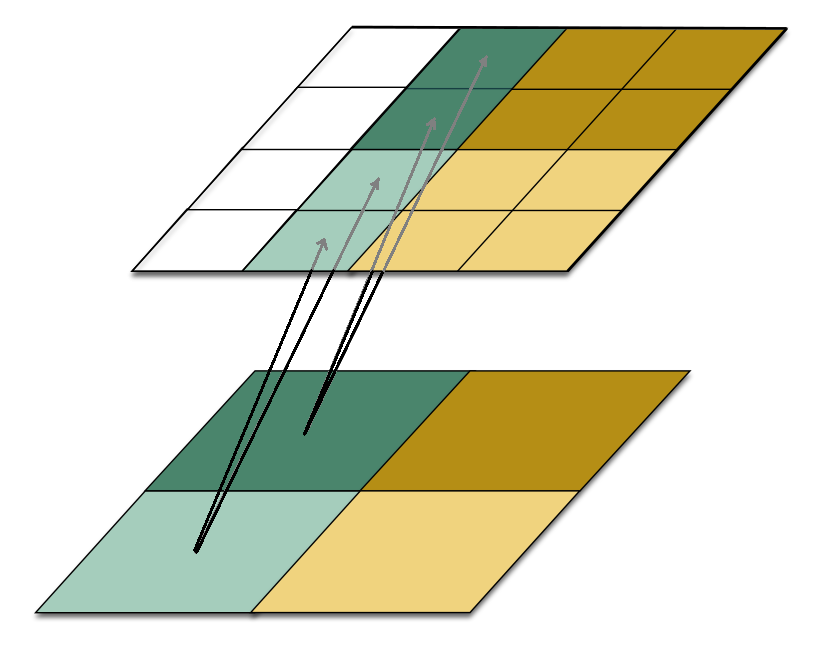
\includegraphics{Images/AMR/refineBoundaryGrid.png}}
  \subfigure[physics kernel execution]
  {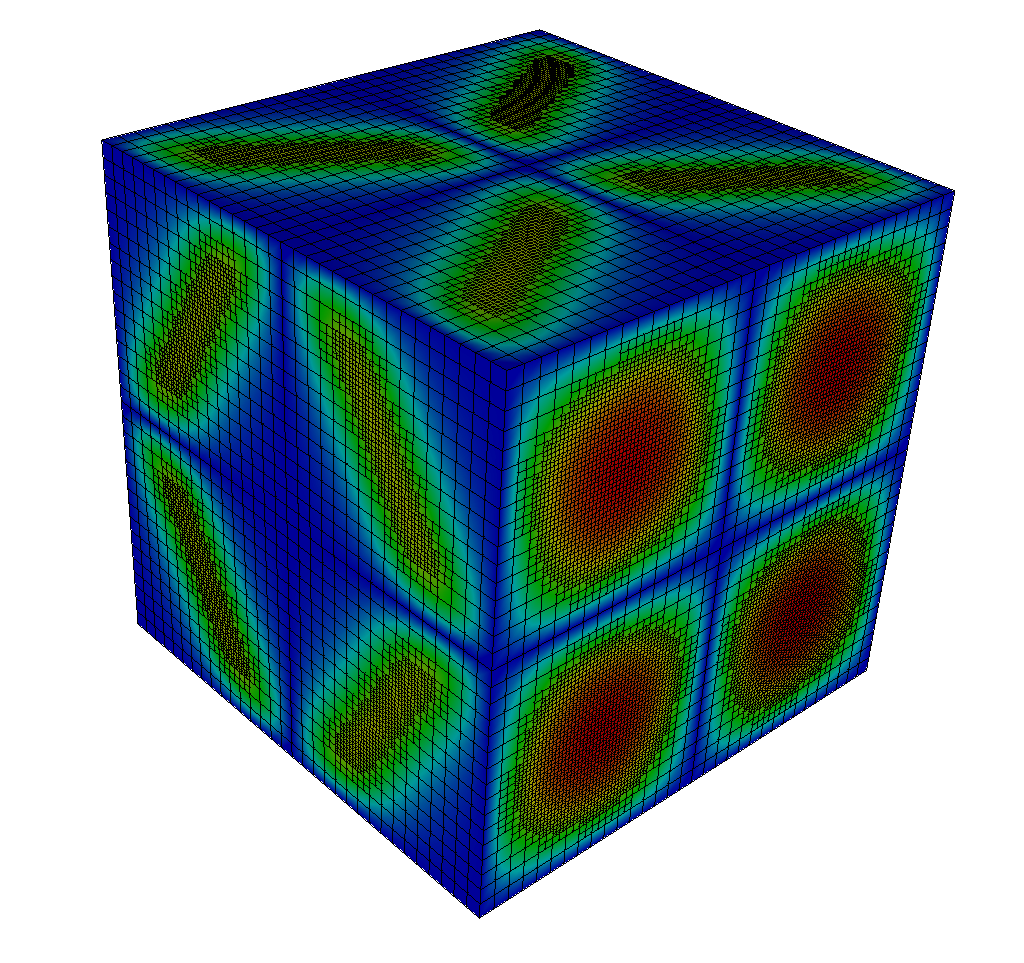
\includegraphics{Images/AMR/taylorgreen_amr0000.png}}
  \subfigure[fine-to-coarse level communication; flux correction on coarse level]
  {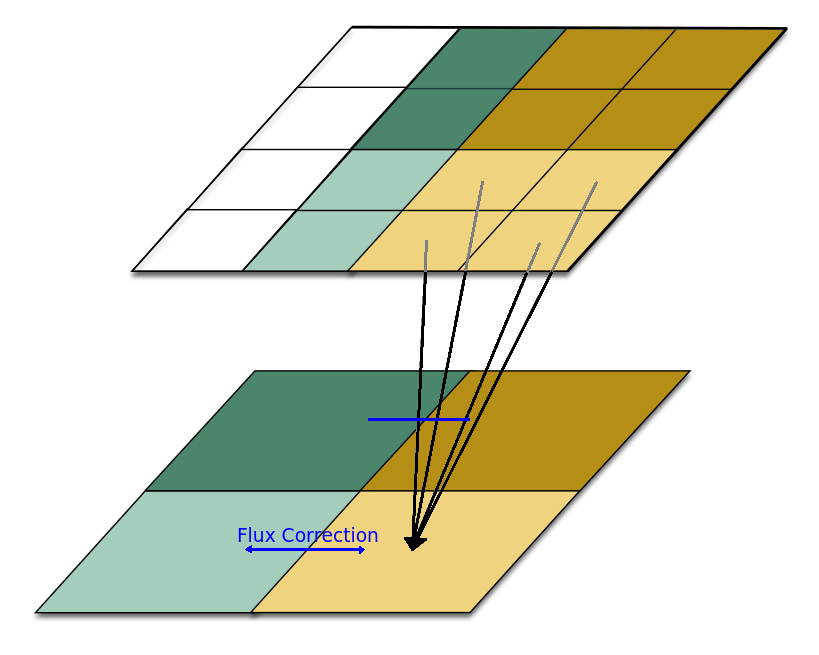
\includegraphics{Images/AMR/coarsen2.png}}
 \end{subfigmatrix}
 \caption{Patch-based AMR communication and solve procedure per computational time step.}
 \label{Patch-AMR-Solve}
\end{figure}




\part{HPC AMR Framework}

\chapter{Overview}
The HPC AMR Framework provides a generalized parallel adaptive mesh refinement infrastructure for arbitrary physics and numerical discretizations. 
This is done by providing three code modules which coordinate adaptive mesh refinement, high-level physics and discretization solver, and low-level numerical kernels. 
To integrate with the HPC AMR Framework, the developer must develop all low-level numerical kernels specific to the physics and discretization 
along with providing appropriate solvers (explicit/implicit, linear/nonlinear, direct/iterative) suitable to the problem.


\subsubsection{Library Dependencies}
The HPC AMR Framework has one direct library dependence which is the \texttt{p4est} AMR software library.
The \texttt{p4est} (\url{http://www.p4est.org/}) software library enables the dynamic management of a collection of adaptive octrees, conveniently called a forest of octrees. \texttt{p4est} is designed to work in parallel and scales to hundreds of thousands of processor cores. It is free software released under GNU General Public License version 2.1 or any later version. 
\medskip

The \texttt{p4est} library has one library dependence which is the \textit{sc} library which is developed and distributed with \texttt{p4est}.
The \texttt{p4est} library does not have any other required library dependencies. 
However, the developer may wish to use external libraries that provide additional capabilities such as \texttt{METIS} for graph partitioning (unstructured grids).
Additionally, \texttt{p4est} uses the adler$32\_$combine function for a parallel checksum which relies on \texttt{zlib} compression in the VTK output routines. 
If configure does not detect this function, it will print a message saying that these features will not work. 
The user can fix this for example by installing \texttt{zlib}'s development binary package, 
or by compiling a current \texttt{zlib} source and pointing the LIBS and CFLAGS environment variables to it. 
The submodule \texttt{sc} also checks for a development version of the \texttt{Lua} library but is not required.


\newpage
\section{Features \& Capabilities}
\begin{itemize}
  \item 2D \& 3D Spatial Dimension Support
  \item Structured \& Unstructured Grid Support
  	\subitem Quad (2D) \& Hex (3D) Elements Only
  \item Periodic Boundary Condition Support For Structured Grids
  \item Embedded Sub-Grids in AMR Elements
    \subitem Arbitrary Number of Elements 
  \item MPI-Enabled Parallel Computations
    \subitem Multiple Ghost Layer Depth Communication Patterns
    \subitem Optional Parallel Grid Partitioning By METIS
  \item Grid Adaption
    \subitem Box Region (static)
    \subitem Point List (dynamic)
    \subitem Feature-Based Physics (dynamic)
  \item Explicit Runge-Kutta (ERK) Time-Stepping Methods For Time-Dependent Problems
  	\subitem ERK1, ERK2, ERK3, ERK4, Low-Storage ERK45
  \item Solution Visualization Through VTK Format
  	\subitem Individual Values at AMR Element Corners
  \item Checkpoint \& Restart 
  	\subitem Automatic Repartitioning of MPI Ranks at Restart
  	\subitem e.g. Initial Simulation (16 MPI Ranks) : Restarted Simulation (32 MPI Ranks)
\end{itemize}





\chapter{Assumptions}
\section{Data Layout}
This framework allows for sub-grids or patches inside of each AMR element.
This is done by allocating a patch-worth amount of data per AMR element and 
then managed by the developer as shown in Fig.~(\ref{subgrids}). In each AMR element, 
a \textbf{one-dimensional pointer} is allocated for the solution storage: 
\begin{eqnarray*}
\textbf{2D} \text{ Simulation}:&  &\texttt{soln}\left( \texttt{NFIELDS},\texttt{NXPATCH},\texttt{NXPATCH} \right) \\
\textbf{3D} \text{ Simulation}:&  &\texttt{soln}\left( \texttt{NFIELDS},\texttt{NXPATCH},\texttt{NXPATCH},\texttt{NXPATCH} \right)
\end{eqnarray*}
where \texttt{NFIELDS} is the number of fields (unknowns) per sub-grid element, 
and \texttt{NXPATCH} is the number of sub-grid elements along one spatial dimension. 
The memory storage ordering (column-major or row-major) is at the discretion of the developer 
since the data storage is allocated as a one-dimensional pointer. Note that all functions developed 
as external solver must be consistent with the memory ordering chosen by the developer.

\begin{figure}[h]
 \begin{subfigmatrix}{4}% number of columns
  \subfigure{}
  \subfigure{\includegraphics{Images/subgrids-2.png}}
  \subfigure{\includegraphics{Images/subgrid-side-array.png}}
    \subfigure{}
 \end{subfigmatrix}
 \caption{Sub-grids in AMR elements: The black elements represent the grid elements represented in \texttt{p4est} 
 and the red elements are the internal sub-grid elements managed by the developer through stacked data storage in each 
 AMR element.}
 \label{subgrids}
\end{figure}

\section{Unstructured Grid Format}
The unstructured grid format that can be read by \texttt{p4est} must be \texttt{ABAQUS} format (see \ref{abaqus-issue}).

\section{Ghost Layer Communication}
The ghost fringe communication width is set to be same as number of sub-grid cells in the AMR element.
This is constrained by the MPI communication pattern of sending entire AMR element solutions to neighboring MPI partitions.
The MPI communication pattern is full connected meaning all neighboring elements touching any face, edge, or corner is communicated (presently). 
Additionally, determining which sub-grid face touches which neighbor element is not currently implemented. 
Thus, the communicated element solution data is invariant to neighboring MPI partitions. 

To change the MPI fringe layer depth, modify the variable \texttt{NFRINGE} in the file \\ \texttt{/hpc/sources/amr/src/var\_defines.h}.
If you modify this variable, you must recompile as it is a run-time constant (required by \texttt{p4est}).

\section{Equation Form}
This framework assumes the governing set of equations are composed into a general left-hand-side (\texttt{lhs}) 
component and a right-hand-side (\texttt{rhs}) component in the form: \texttt{lhs} = \texttt{rhs}.
The function physics\_rhs\_\{un\}structured() is responsible for constructing the \texttt{rhs} of the discretized 
set of equations. To demonstrate this concept, we present two cases.
\bigskip

\noindent \textbf{Structural Stiffness Equation}: \\
The discrete equations from structural analysis is written as follows:
\begin{equation*}
\left[\mathbf{K} \right] \mathbf{u} - \mathbf{f} = 0
\end{equation*}
where $\left[\mathbf{K} \right]$ is the global element stiffness matrix, 
$\mathbf{u}$ is the unknown node displacement vector, and 
$\mathbf{f}$ is the node force vector. The equation in the proper form:
\begin{equation*}
\underbrace{\left[\mathbf{K} \right] \mathbf{u}}_{\texttt{lhs}} = \underbrace{\mathbf{f}}_{\texttt{rhs}}
\end{equation*}
Following the construction of the right hand side, the developer is then responsible of solving the final set of equations 
\texttt{lhs} = \texttt{rhs} by appropriate means, e.g. this example might use a direct method or a sparse iterative method 
to solve for the unknown vector $\mathbf{u}$.
\bigskip

\noindent \textbf{Advection Equation}: \\
The governing equation for advection is written as follows:
\begin{equation*}
\frac{\partial\psi}{\partial t} + \nabla\cdot\left( \psi{\mathbf{u}}\right) = 0 
\end{equation*}
where $\mathbf{u}$ is the velocity field and $\psi$ is conserved scalar field. Then we rearrange the equation and define the left-hand-side and the right-hand-side:  
\begin{equation*}
\underbrace{\frac{\partial\psi}{\partial t}}_{\texttt{lhs}} = \underbrace{-\nabla\cdot\left( \psi{\mathbf{u}}\right)}_{\texttt{rhs}}
\end{equation*}
As this is a time-dependent problem, some explicit time integrators are provided in the framework to solve this type of set of equations, i.e. the left-hand-side is the continuous temporal derivative of the unknown quantity and the right-hand-side is the discrete spatial residual.


\newpage
\chapter{Source Code Organization}
The HPC AMR Framework is composed of three modules: \textbf{amr}, \textbf{physics}, and \textbf{solver}.
The source code directory is structured as follows:
\begin{verbatim}
hpc/
  docs
  sources/
    amr/
      src
    physics/
      src
    solver/
      src
\end{verbatim}

\noindent
\underline{\textbf{amr}}: 
The amr module is responsible for the top-level simulation driving functionality:
\begin{itemize}
\item evolve, checkpoint, visualize, and grid adaption
\item Fig.~(\ref{main}) demonstrates the call graph of the amr::\inltt{main()} function.
\end{itemize}

\noindent
\underline{\textbf{physics}}:
The physics module is responsible for the top-level physics and numerical discretization:
\begin{itemize}
\item Physics Interfaces: physics and solver setup
\item Numerical Discretization Solve: explicit/implicit solvers, MPI communication
\item Fig.~(\ref{evolve}) demonstrates the call graph of the physics::\inltt{hpc\_amr\_evolve\_solver()} function.
\end{itemize}

\noindent
\underline{\textbf{solver}}: The solver module is responsible for the low-level numerical discretization kernels:
\begin{itemize}
\item volume, face, edge, corner residual kernels
\item The right-most column of Fig.~(\ref{evolve}) call graph shows the primary numerical kernels in the solver module.
\end{itemize}

\noindent
The developer is responsible for providing all functions in the solver module and the explicit/implicit solver in the physics module.
Chapter~\ref{development-procedure} outlines the specific functions required from the developer to integrate their physics and numerical discetization.
For time-dependent problems in Method-of-Lines form $\frac{\partial Q}{\partial t} = R$, some explicit time integrators are provided.

\begin{figure}
 \begin{subfigmatrix}{2}% number of columns
  \subfigure{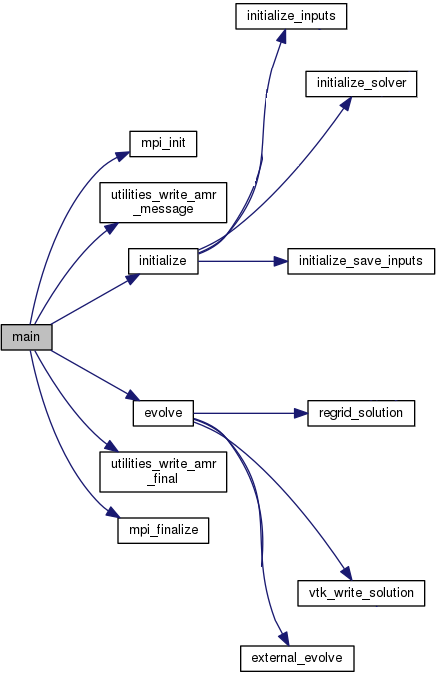
\includegraphics{Images/amr-1.png}}
 \end{subfigmatrix}
 \caption{Call graph of AMR::main()}
 \label{main}
\end{figure}

\begin{landscape}
\begin{figure}
 \begin{subfigmatrix}{1}% number of columns
  \subfigure{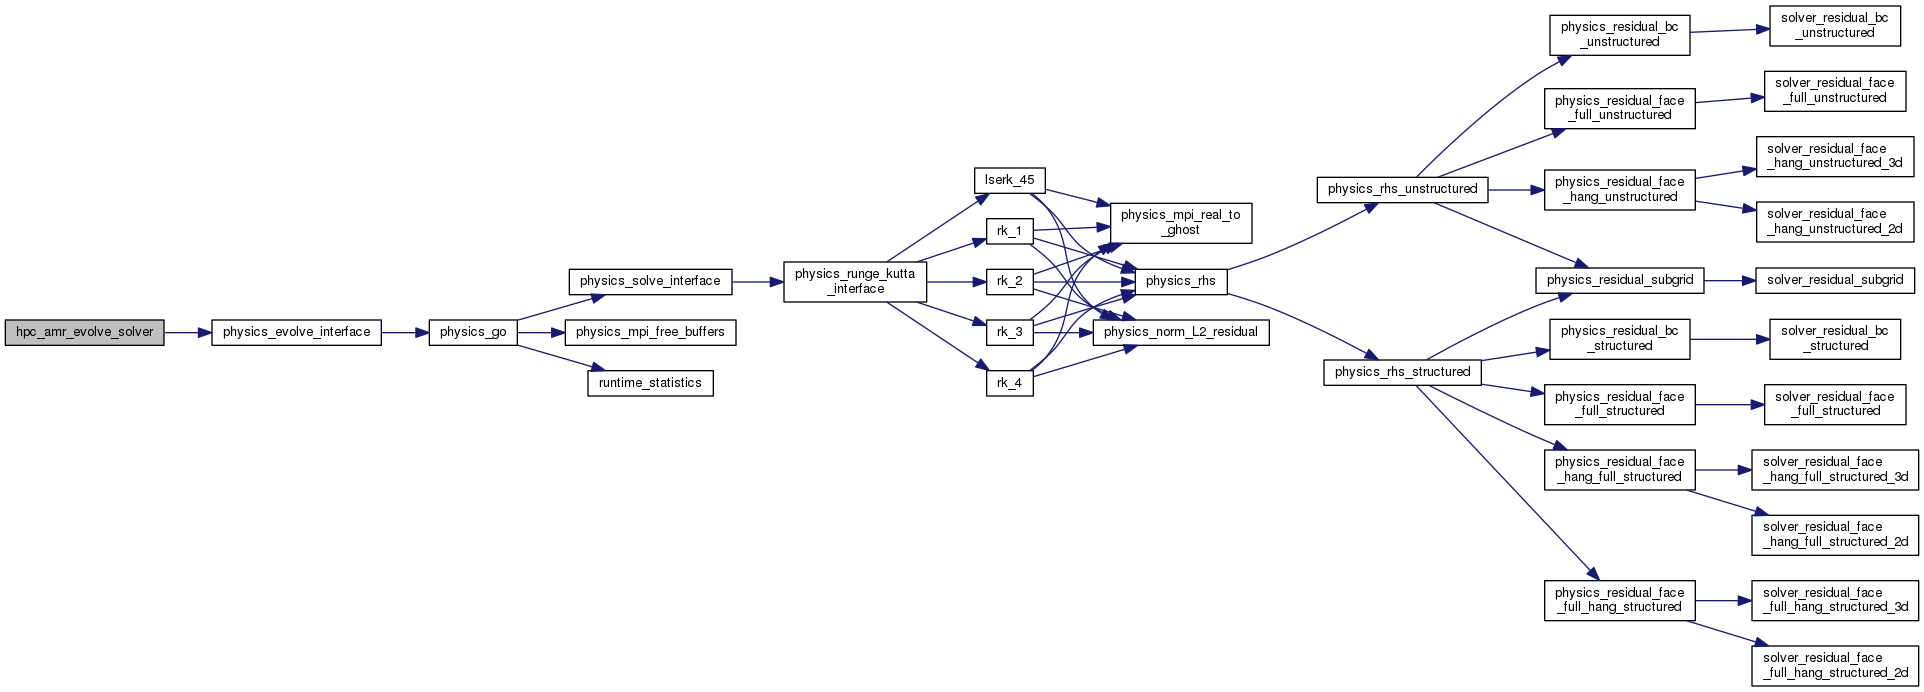
\includegraphics{Images/evolve-call-graph.png}}
 \end{subfigmatrix}
 \caption{Call graph of PHYSICS::hpc\_amr\_evolve\_solver() function called from AMR::external\_evolve(). The last column of functions (right) belong to the SOLVE code module which are the primary numerical kernels implemented by the developer.}
 \label{evolve}
\end{figure}
\end{landscape}



\chapter{External Solver Development}\label{development-procedure}
\section{Procedure Summary}
\begin{itemize}
\item Modify \texttt{hpc/sources/amr/src/var\_defines.h}
  \subitem --Set \texttt{NFRINGE} to required number of MPI ghost layers 
  \subitem --Set \texttt{NFIELDS} to required number of fields (unknowns) per grid point 
\item Implement physics and solver functions related to numerical discretization
  \subitem --Read and setup user inputs: physics-related variables, solver-related variables, etc.
\item Implement general and grid-specific physics residual functions outlined in \ref{general-functions}, \ref{structured-functions}, \ref{unstructured-functions}
  \subitem --Example functions provided in \texttt{hpc/sources/solver/src/}
\item Implement solver interface \inltt{physics\_?\_interface} and solver outlined in \ref{solver-functions}
  \subitem --Explicit/Implicit/Direct/Iterative solver for \texttt{lhs} = \texttt{rhs}
  \subitem -- -- e.g. solve $\left[ \mathbf{K} \right] \mathbf{u} = \mathbf{f}$ with sparse iterative method
  \subitem --Analogous to \inltt{physics\_runge\_kutta\_interface} and \inltt{rk\_?}
  \subitem -- -- Example \inltt{physics\_runge\_kutta\_interface} located in \texttt{hpc/sources/physics/src}
  \subitem -- -- Example \inltt{rk\_?} located in \texttt{hpc/sources/physics/src/rk\_time\_integrators.c}
\end{itemize}


\section{Procedure Details}
The HPC AMR Framework provides the infrastructure to calculate \texttt{rhs} on structured and unstructured adaptive grids in 2D and 3D. 
To implement new physics and numerical discretization kernels into the framework, the developer is responsible for the numerical kernels that correspond to the right-most column of functions in Fig.~(\ref{evolve}) in addition to a physics solver which will solve a set of equations in the form \texttt{lhs} = \texttt{rhs}, where \texttt{lhs} contains the unknown solution vector and functional operator, e.g. $\left[ \mathbf{K} \right] \mathbf{u}$, and \texttt{rhs} is the spatial residual of the equation, e.g. $\mathbf{f}$. 
For time accurate problems in Method-of-Lines form $\frac{\partial Q}{\partial t} = R$, some explicit time integration schemes are available within the framework including various explicit Runge-Kutta methods. 
\bigskip

\noindent
A list of the functions required by the developer are as follows (2D and/or 3D):


\subsection{General Functions}\label{general-functions}
\begin{itemize}
\item \inltt{solver$\_$initialize$\_$quadrant(...)}: Initialize solution data in each AMR element
\item \inltt{solver$\_$residual$\_$subgrid(...)}: Calculate total residual of sub-grid in each AMR element
  \subitem --Volume/Face/Edge/Node residual kernels depending on numerical discretization
\item \inltt{solver$\_$refine$\_$operator$\_$?d(...)}: Refinement Operator: coarse solution to fine solutions
\item \inltt{solver$\_$coarsen$\_$operator$\_$?d(...)}: Coarsen Operator: Fine solutions to coarse solution  
\item \inltt{solver$\_$visualize$\_$quad(...)}: Interpolate sub-grid solution to corners of AMR element
\item \inltt{solver$\_$tag$\_$feature(...)}: AMR feature tagging method for refinement
\item \inltt{physics$\_$regrid$\_$points(...)}: Read list of points (x,y,z,h) for AMR regridding
\end{itemize}


\subsection{Structured Grids}\label{structured-functions}
In addition to the general functions, structured grid numerical kernels:

\begin{itemize}
\item \inltt{solver$\_$residual$\_$bc$\_$structured(...)}: Grid boundary condition residual 
\item \inltt{solver$\_$residual$\_$face$\_$full$\_$structured(...)}: Residual at full element face (no hanging faces)
\item \inltt{solver$\_$residual$\_$face$\_$full$\_$hang$\_$structured(...)}: Residual at hanging element face
  \subitem Right elements are one level finer than left element% as shown Fig.~(\ref{hang-elements})(a)
\item \inltt{solver$\_$residual$\_$face$\_$hang$\_$full$\_$structured(...)}: Residual at hanging element face
  \subitem Left elements are one level finer than right element% as shown Fig.~(\ref{hang-elements})(b)
\end{itemize}
		

\subsection{Unstructured Grids}\label{unstructured-functions}
In addition to the general functions, unstructured grid numerical kernels:

\begin{itemize}
\item \inltt{solver$\_$residual$\_$bc$\_$unstructured(...)}: Grid boundary condition residual
\item \inltt{solver$\_$residual$\_$face$\_$full$\_$unstructured(...)}: Residual at full element face
\item \inltt{solver$\_$residual$\_$face$\_$hang$\_$unstructured(...)}: Residual at hanging element face
\end{itemize}


%\begin{figure}
% \begin{subfigmatrix}{2}% number of columns
%  \subfigure[Full-hang face]{\includegraphics{Images/full-hang-face.png}}
%  \subfigure[Hang-full face]{\includegraphics{Images/hang-full-face.png}}
% \end{subfigmatrix}
% \caption{Structured grid non-conforming element types.}
% \label{hang-elements}
%\end{figure}
%\bigskip

\subsection{Explicit/Implicit/Direct/Iterative Solvers}\label{solver-functions}
Implementation of solvers is required as necessary to the discretized equations. 
For example, to solver the problem $[K]u = f$ where $[K]$ is a sparse matrix, 
either a direct method or iterative method can be used to solve the problem.
\begin{itemize}
\item Solver interface should imitate \inltt{physics\_runge\_kutta\_interface} function
\item Solver should imitate \inltt{rk\_1} function
\end{itemize}

\newpage
\section{An In-Depth Look -- Physics::physics\_rhs\_unstructured()}
To provide context of the AMR element and solution data structures, we provide a line-by-line look at the Physics code module function \inltt{solver$\_$residual$\_$unstructured(...)} located in \texttt{hpc/sources/physics/src/physics\_rhs\_unstructured.c} (the structured grid residual function is analogous).

\subsection*{Function Declaration}
\begin{lstlisting}[language=c]
void physics_rhs_unstructured(
	int *dim, 
	int *nfields, 
	int *nelem_subgrid,
	int *ncell, 
	int *cell_info, 
	double *geom, 
	int *nface, 
	int *face_info,
	int *dof, 
	double *soln, 
	double *rhs)
\end{lstlisting}


\subsubsection{Arguments}
\begin{itemize}[label={}]
\item \inltt{int *dim} : simulation spatial dimension
  \subitem e.g. 3D simulation $\rightarrow$ *dim = 3
\item \inltt{int *nfields} : number of fields (unknowns) per grid point define by physics
  \subitem e.g. 3D conservative fluid variables (mass, momentum, energy) $\rightarrow$ *nfields = 5
\item \inltt{int *nelem\_subgrid} : number of 1D sub-grid elements in an AMR element
  \subitem e.g. Fig.~(\ref{subgrids}) has 4 by 4 elements in each AMR element $\rightarrow$ *nelem\_subgrid = 4
\item \inltt{int *ncell} : number of real (non-ghost) AMR cells in the soln/rhs pointer arrays 
\item \inltt{int *cell\_info}[3*ncell] : AMR data structure information related to the AMR cells
  \subitem cell\_info[0] = cell type (assigned by user to indicate specific cell indicator, e.g. cut-cell)
  \subitem cell\_info[1] = cell grid level
  \subitem cell\_info[2] = cell solution index into \texttt{*soln} and \texttt{*rhs} pointer
\end{itemize}

\newpage
\begin{itemize}[label={}]
\item \inltt{double *geom} : AMR cell geometry coordinates (corners)
  \subitem The cell corner coordinates are listed with $x-, y-, z-$components 
  (2D also has three components listed with $z=0.0$) with node ordering as follows (see \ref{appendix:AMR-ref-coordinates}):\\
  \begin{verbatim}
          2D Reference Element:                       3D Reference Element:

                                            n3 o------------o n4
n3 o-----------o n4                           /|           /|     n1 = (-1,-1,-1)
   |           |      n1 = (-1,-1, 0)        / |          / |     n2 = ( 1,-1,-1)
   |           |      n2 = ( 1,-1, 0)       /  |         /  |     n3 = (-1, 1,-1)
   |           |      n3 = (-1, 1, 0)   n7 o------------o n8|     n4 = ( 1, 1,-1)
   |           |      n4 = ( 1, 1, 0)      |n1 o--------|---o n2  n5 = (-1,-1, 1)
n1 o-----------o n2                        |  /         |  /      n6 = ( 1,-1, 1)
                                           | /          | /       n7 = (-1, 1, 1)
                                           |/           |/        n8 = ( 1, 1, 1)
                                        n5 o------------o n6
  \end{verbatim}
   
\item \inltt{int *nface} : number of AMR element faces to compute face residual kernel
\item \inltt{int *face\_info}[11*nface] : AMR data structure information related to the AMR cell faces
  \subitem face\_info[0] = face type
  \subitem \hspace{1cm} face type = 1 $\rightarrow$ boundary face (no neighbor element)
  \subitem \hspace{1cm} face type = 2 $\rightarrow$ full face
  \subitem \hspace{1cm} face type = 3 $\rightarrow$ 2D hanging face 
  \subitem \hspace{1cm} face type = 5 $\rightarrow$ 3D hanging face 
  \subitem face\_info[1] \ = side of AMR element -- see \ref{appendix:AMR-ref-sides}
  \subitem face\_info[2] \ = AMR element owner cell index into cell\_info
  \subitem face\_info[3] \ = AMR element neighbor 1 cell index in cell\_info (if present)
  \subitem face\_info[4] \ = AMR element neighbor 2 cell index in cell\_info (if present)
  \subitem face\_info[5] \ = AMR element neighbor 3 cell index in cell\_info (if present)
  \subitem face\_info[6] \ = AMR element neighbor 4 cell index in cell\_info (if present)
  \subitem face\_info[7] \ = AMR element neighbor 1 side  (if present)
  \subitem face\_info[8] \ = AMR element neighbor 2 side  (if present)
  \subitem face\_info[9] \ = AMR element neighbor 3 side  (if present)
  \subitem face\_info[10] = AMR element neighbor 4 side  (if present)
\item \inltt{int *dof} : number of real (non-ghost) degrees of freedom (length of \texttt{*rhs})
\item \inltt{double *soln}[nfields*(nelem\_subgrid**dim)*(ncell+nghost)] : solution data pointer
  \subitem Real and Ghost data are stacked in this pointer 
  \subitem Real solution data starts at \texttt{soln[0]}; Ghost data starts at \texttt{soln[dof]}
\item \inltt{double *rhs}[nfields*(nelem\_subgrid**dim)*(ncell)] : right-hand-side equation data pointer
\end{itemize}




\newpage
\subsection*{Function Body: Physics::physics\_rhs\_unstructured()}
\noindent 
\underline{Lines 66-70}:
\begin{verbatim}
    ncorners = 4;
    if(*dim==3){
        ncorners = 8;
    }
    ncorners *= 3; // multiply in 3 coordinates per node (2D also)
\end{verbatim}
We are assigning the number of corner points times the number of coordinates per point. Thus, for 2D quads, there are four corners per quad and three coordinates per corner (x, y, z) setting \texttt{ncorners = 12}.
\bigskip

\noindent 
\underline{Lines 74-77}:
\begin{verbatim}
    /* zero the rhs */
    for(i = 0; i < *dof; i++){
        rhs[i] = 0.0;
    }
\end{verbatim}
As indicated by the comment, we are zeroing the \texttt{rhs} vector for all the real degrees of freedom which there are \texttt{*dof} number of them.
\bigskip

\noindent 
\underline{Lines 80-91}:
\begin{verbatim}
    /* face loop - compute face residual */
    for(face_id = 0; face_id < *nface; face_id++){
        
        /* this cell's information */
        face_index = d_physics_interface.extern_face_size*face_id;
        facetype    = face_info[face_index+0];
        side_l      = face_info[face_index+1];
        cell_l      = face_info[face_index+2];
        
        cell_index  = d_physics_interface.extern_cell_size*cell_l;
        type_l      = cell_info[cell_index+0];
        ind_l       = cell_info[cell_index+2];
        
         switch (facetype){
            ...
         }
    }
\end{verbatim}
This is the face loop which is responsible for calculating the spatial residual contribution from element faces.
The loop iterates over the total number of AMR element faces \texttt{*nfaces}. 
The variable \texttt{face\_index} assigns the index into the \texttt{face\_info} data structure where 
\texttt{d\_physics\_interface.extern\_face\_size} 
is the number of fields per face which is 11 as outlined in function declaration section above. 
The following variable assignments access the face info data structure assigning the AMR element owner information 
(each face is assigned a unique AMR element owner). 
Once the \texttt{face\_type} is established, the proper residual function is called in lines 94-187.
\bigskip
\bigskip

\noindent 
\underline{Lines 94-187}:
\begin{verbatim}
        switch (facetype){
            
            case 1:
                /* mesh boundary --> cell is real */
                ...
                physics_residual_bc_unstructured(...);
                break;
                
            case 2: 
                /* full-full --> check both if real or ghost */
                ...
                physics_residual_face_full_unstructured(...);
                break;
                
            case 3:
                /* hanging 2D --> check all if real or ghost: ind > dof = ghost */
                ...
                physics_residual_face_hang_unstructured(...);
                break;
                
            case 5:
                /* hanging 3D --> check all if real or ghost: ind > dof = ghost */
                ...
                physics_residual_face_hang_unstructured(...);
                break;
                
        }                
\end{verbatim}
Case 1: face is on grid boundary requiring a boundary condition residual computation\\
Case 2: face is an interior grid face with equal size AMR elements on each side of the face\\
Case 3: face is a 2D hanging face; adjoining elements are on two different consecutive AMR levels\\
Case 5: face is a 3D hanging face; adjoining elements are on two different consecutive AMR levels
\bigskip

\noindent
We will examine each case in detail.
\newpage

\noindent
\underline{Case 1: Lines 96-109}:
\begin{verbatim}
            case 1:
                /* mesh boundary --> cell is real */
                
                //TODO: assign bc type
                //TODO: ...
                bc = type_l;
                
                physics_residual_bc_unstructured(dim,nfields,nelem_subgrid,
                                                 &side_l,&type_l,&bc,
                                                 &geom[ncorners*cell_l],
                                                 &soln[ind_l],&rhs[ind_l]);
                
                break;
\end{verbatim}
As noted in the comments, the boundary condition flag indicator should be set. 
For this example, the cell element type is used to indicate the type of boundary condition that should be calculated.
The variable \texttt{side\_l} (see \ref{appendix:AMR-ref-sides}) indicates which sub-grid array face to modify.
\medskip

\noindent
\underline{Case 2: Lines 111-131}:
\begin{verbatim}
            case 2: 
                /* full-full --> check both if real or ghost */
                
                /* full neighbor's information */
                cell_r[0]   = face_info[face_index+3];
                side_r[0]   = face_info[face_index+7];
                type_r[0]   = cell_info[d_physics_interface.extern_cell_size*cell_r[0]+0];
                ind_r[0]    = cell_info[d_physics_interface.extern_cell_size*cell_r[0]+2];
                
                
                physics_residual_face_full_unstructured(
                    dim,nfields,nelem_subgrid,
                    &side_l,&side_r[0],
                    &type_l,&type_r[0],
                    &ind_l,&ind_r[0],dof,
                    &geom[ncorners*cell_l],
                    &geom[ncorners*cell_r[0]],
                    &soln[ind_l],&soln[ind_r[0]],
                    rhs);
                
                break;
\end{verbatim}
This case is a full interior face. The neighbors AMR element information is gathered as passed as function arguments. 
It should noted that we need to check if either cell is a ghost, and, therefore, skip writing into the \texttt{rhs} pointer 
since the ghost ind\_r value will be longer than the \texttt{rhs} array thereby causing an out-of-bounds error.
\newpage


\noindent
\underline{Case 3: Lines 133-154}:
\begin{verbatim}
            case 3:
                /* hanging 2D --> check all if real or ghost: ind > dof = ghost */
                
                /* hanging neighbors' information */
                cell_r[0]   = face_info[face_index+3];
                cell_r[1]   = face_info[face_index+4];
                side_r[0]   = face_info[face_index+7];
                side_r[1]   = face_info[face_index+8];
                type_r[0]   = cell_info[d_physics_interface.extern_cell_size*cell_r[0]+0];
                type_r[1]   = cell_info[d_physics_interface.extern_cell_size*cell_r[1]+0];
                ind_r[0]    = cell_info[d_physics_interface.extern_cell_size*cell_r[0]+2];
                ind_r[1]    = cell_info[d_physics_interface.extern_cell_size*cell_r[1]+2];
                
                physics_residual_face_hang_unstructured(
                    dim,nfields,nelem_subgrid,
                    &side_l,&side_r[0],
                    &type_l,&type_r[0],
                    &cell_l,&cell_r[0],
                    &ind_l,&ind_r[0],
                    dof,geom,soln,rhs);
                
                break;
\end{verbatim}
This case is a 2D non-conforming element hanging face scenario. The two hanging neighbor AMR elements' information are assigned into pointers and passed as function arguments. The \texttt{cell\_r} pointer is the cell indexes into the \texttt{cell\_info} pointer, \texttt{side\_r} are the AMR element reference side indexes (which is used to determine the subgrid array indexes and face normal vectors if performing a structured grid calculation -- see \ref{appendix:AMR-ref-sides}), \texttt{type\_r} are the AMR cell types, and \texttt{ind\_r} are the solution array (\texttt{soln}) indexes for each of the neighboring AMR cells. Note that when calculating the residual, check all element indexes to assert they are real AMR elements on this MPI rank, otherwise an out-of-bounds error will occur. To do this check, simply assert (\texttt{ind\_}? $<$ \texttt{dof}) before writing into \texttt{rhs}.
\newpage


\noindent
\underline{Case 5: Lines 156-185}:
\begin{verbatim}
            case 5:
                /* hanging 3D --> check all if real or ghost: ind > dof = ghost */
                
                /* hanging neighbors' information */
                cell_r[0]   = face_info[face_index+3];
                cell_r[1]   = face_info[face_index+4];
                cell_r[2]   = face_info[face_index+5];
                cell_r[3]   = face_info[face_index+6];
                side_r[0]   = face_info[face_index+7];
                side_r[1]   = face_info[face_index+8];
                side_r[2]   = face_info[face_index+9];
                side_r[3]   = face_info[face_index+10];
                type_r[0]   = cell_info[d_physics_interface.extern_cell_size*cell_r[0]+0];
                type_r[1]   = cell_info[d_physics_interface.extern_cell_size*cell_r[1]+0];
                type_r[2]   = cell_info[d_physics_interface.extern_cell_size*cell_r[2]+0];
                type_r[3]   = cell_info[d_physics_interface.extern_cell_size*cell_r[3]+0];
                ind_r[0]    = cell_info[d_physics_interface.extern_cell_size*cell_r[0]+2];
                ind_r[1]    = cell_info[d_physics_interface.extern_cell_size*cell_r[1]+2];
                ind_r[2]    = cell_info[d_physics_interface.extern_cell_size*cell_r[2]+2];
                ind_r[3]    = cell_info[d_physics_interface.extern_cell_size*cell_r[3]+2];
                
                physics_residual_face_hang_unstructured(
                    dim,nfields,nelem_subgrid,
                    &side_l,&side_r[0],
                    &type_l,&type_r[0],
                    &cell_l,&cell_r[0],
                    &ind_l,&ind_r[0],
                    dof,geom,soln,rhs);
                
                break;
\end{verbatim}
This case is analogous to Case 3 above; this scenario is the 3D non-conforming element hanging face. There are four neighboring AMR elements on one side of the face and one AMR element on the other. The cell indexes, sides, types, and solution indexes are assigned as passed as arguments. 
Note that when calculating the residual, check all element indexes to assert they are real AMR elements on this MPI rank, otherwise an out-of-bounds error will occur. To do this check, simply assert (\texttt{ind\_}? $<$ \texttt{dof}) before writing into \texttt{rhs}.

\newpage

\noindent
\underline{Lines 192-203}:
\begin{verbatim}
    /* element loop: compute cell subgrid face, volume, source term residuals */
    for(cell_id = 0; cell_id < *ncell; cell_id++){
        
        cell_index = d_physics_interface.extern_cell_size*cell_id;
        type    = cell_info[cell_index+0];
        level   = cell_info[cell_index+1];
        cell    = cell_info[cell_index+2];
        
        physics_residual_source (dim,nfields,nelem_subgrid,&type_l,
                                 &geom[ncorners*cell_id],&soln[cell],&rhs[cell]);
        physics_residual_subgrid(dim,nfields,nelem_subgrid,&type,&level,
                                 &geom[ncorners*cell_id],&soln[cell],&rhs[cell]);
        
    }
\end{verbatim}
This is the element loop which is responsible for calculating the spatial residual contribution from element volumes and all sub-grid residual calculations which may also include sub-grid face/edge/node residual contributions.
The loop iterates over the total number of AMR elements \texttt{*ncell}. 
Within this loop, source terms may also be added to the \texttt{rhs} array.
\medskip

\noindent
\underline{Lines 205-208}:
\begin{verbatim}
    /* rhs = -R */
    for(i = 0; i < *dof; i++){
        rhs[i] *= -1.0;
    }
\end{verbatim}
This example is solving for the right-hand-side of the equation $\frac{\partial Q}{\partial t} = -R\left(Q\right)$. 
The numerical kernels in this example construct $+R\left(Q\right)$. Thus, for our \texttt{rhs} pointer to be of the correct sign, we multiply all entries by negative one. 
\bigskip

\noindent 
\textbf{TIP}: We multiply the \texttt{rhs} pointer at the end by a negative sign to be explicit and clear in the physics calculations. This is helpful for more complicated discretization scenarios such as when using a Newton-Ralphson method where we need to calculate the Jacobian matrix of $+R\left(Q\right)$. If we bury the negative sign into the residual $R$, we may inadvertently calculate the Jacobian matrix of $-R\left(Q\right)$.


\chapter{Framework Documentation \& Example}

\section{Source Code Documentation}
Source code documentation is provided via Doxygen. The Doxygen configuration file is located in \texttt{hpc/docs} and is named \texttt{Doxyfile}. You will need Graghviz installed to properly generate all the call graphs. To generate the documents from the command-line: \texttt{doxygen Doxyfile}

Doxygen will generate a directory named \texttt{ouput} which two subdirectories: \texttt{html} and \texttt{latex}. To view the source code documentation via your web browser, open the \texttt{html/index.html} file with your web browser.

\section{Example Solver}
An example Computational Fluid Dynamics solver is provided as demonstration of integration with the HPC AMR Framework.
The source code of the example solver is provided in \texttt{hpc/sources/solver/src}. 
There are structured and unstructured grid functionality examples in 2D and 3D provided. 
The solver is a first-order Finite Volume method for the conservative compressible inviscid flow equations.




\chapter{Known Issues}
\section{Unstructured Grid Format: \texttt{ABAQUS} .inp}\label{abaqus-issue}
\subsection{\texttt{*ELEMENT} Header Sections}
There is an issue with reading \texttt{ABAQUS} .inp  format with \texttt{p4est}; 
when \texttt{p4est} searches for the element connectivity in the grid file, it 
searches for \texttt{*ELEMENT}. There may be more than one section with the 
\texttt{*ELEMENT} header. This will cause a \texttt{p4est} error stating there 
are more elements than listed. \textbf{There must only be one \texttt{*ELEMENT} section.}

\subsection{Element ID Numbering}
In addition to the element headers, the element numbering is anticipated to start 
at index 1 as the following demonstrates:
\begin{verbatim}
************************** E L E M E N T S **************************
*ELEMENT, TYPE=S4R, ELSET=EB1
       1,       1,       2,     111,      73
       2,       2,       3,     110,     111
       3,       3,       4,     109,     110
       4,       4,       5,      74,     109
       5,       5,       6,      75,      74
       6,       6,       7,      76,      75
\end{verbatim}
However, sometimes the generated \texttt{ABAQUS} format writes the element id starting 
at some arbitrary integer. When \texttt{p4est} reads the file, it uses the element id 
to index its grid storage array. This will cause an error stating 
\begin{verbatim}
[p4est 0] Encountered element that will not fit into tree_to_vertex array. 
[p4est 0] More elements than expected.
[p4est 0] Failed to read ?.inp: pass 2
\end{verbatim}
\textbf{Element id numbering must start at 1 and be consecutively numbered.}

\newpage
\section{METIS Partitioning After Adaption}
The use of METIS for graph partitioning is beneficial for unstructured meshes 
as \texttt{p4est} uses a \textit{z-ordering} (also known as Morton Ordering) approach for binary trees. 
However this approach does not work well for unstructured meshes which has each 
element registered as a tree in the AMR forest. METIS is able to place neighboring 
unstructured elements on the same processor allowing for much better parallel communication 
patterns. 

There is an issue when partitioning after performing mesh adaption on an unstructured grid.
It appears that \texttt{p4est} performs the partitioning with the \textit{z-ordering} 
approach even though the initial grid uses METIS for partitioning. This causes AMR elements 
to be scattered amongst parallel processes as seen in Fig.~(\ref{unstructured-mpi}) 
causing excessive communication patters which increases the parallel communication 
time up to 20\% of the total simulation. 


\begin{figure}
 \begin{subfigmatrix}{2}% number of columns
  \subfigure[before grid adaption]{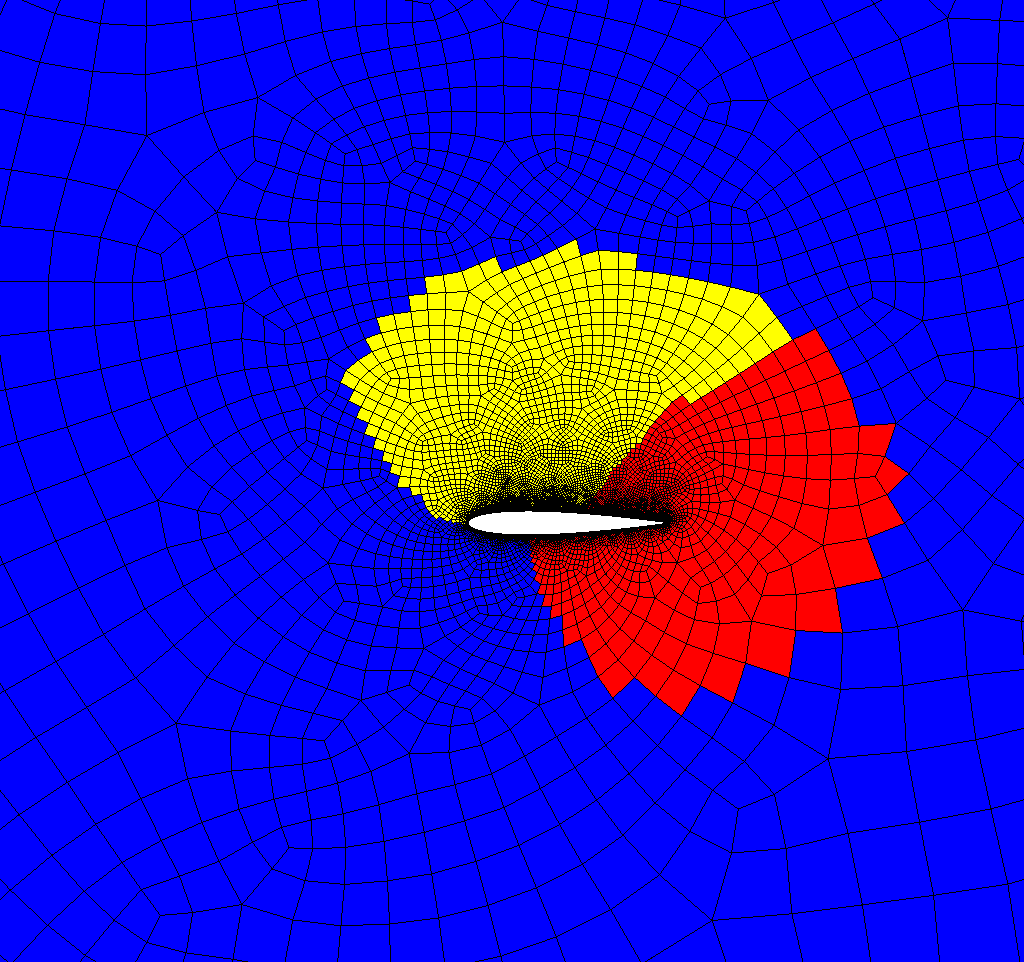
\includegraphics{Images/unstructured-mpi-ranks-before.png}}
  \subfigure[after grid adaption]{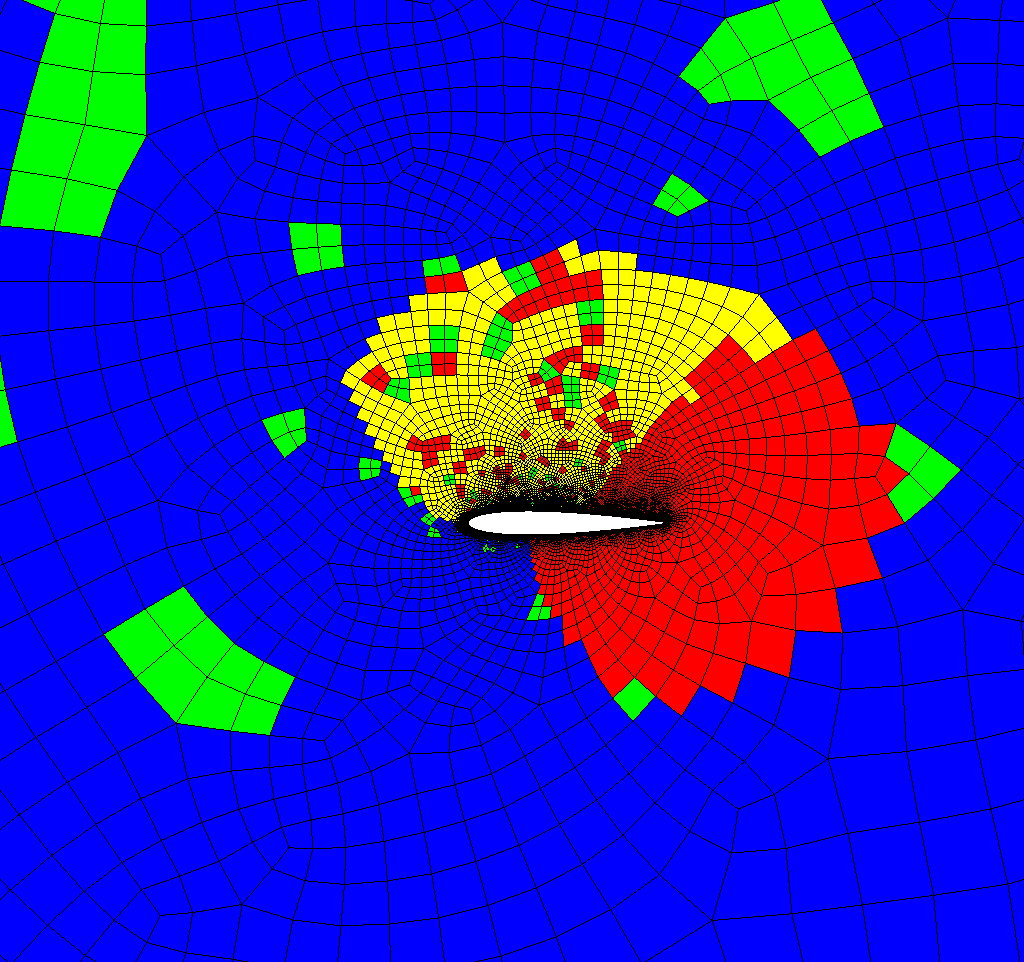
\includegraphics{Images/unstructured-mpi-ranks-after.png}}
 \end{subfigmatrix}
 \caption{MPI ranks on unstructured grid.}
 \label{unstructured-mpi}
\end{figure}


\section{AMR Grid Coarsening Run-to-Run Consistency}
The coarsening processing is inconsistent run-to-run with no input changes even when using one mpi rank.
The number of cells on each AMR level may not be the same as previous runs when allowing AMR grid coarsening.
This will result in regression test failure because the problem has changed.

However, when AMR grid coarsening is disabled (\texttt{hpc/sources/amr/src/amr\_evolve.c}: Line 53, set to 0),
the run-to-run comparison of AMR element counts and residual checks are consistent. Thus, it is recommended to 
build and run all regression tests with dynamic grid adaption, coarsening should be disabled.



\newpage
\begin{appendices}\label{appendix}
\chapter{Reference Elements}
\section{AMR Element Coordinates Ordering}\label{appendix:AMR-ref-coordinates}
The AMR element corner coordinates are listed with $x-, y-, z-$components (2D also has three components with $z=0.0$) with node ordering as follows:
\begin{verbatim}
2D Reference Element:                      3D Reference Element:
---------------------                      ---------------------
                                             n3 o------------o n4
n3 o-----------o n4                            /|           /|     n1 = (-1,-1,-1)
   |           |       n1 = (-1,-1, 0)        / |          / |     n2 = ( 1,-1,-1)
   |           |       n2 = ( 1,-1, 0)       /  |         /  |     n3 = (-1, 1,-1)
   |           |       n3 = (-1, 1, 0)   n7 o------------o n8|     n4 = ( 1, 1,-1)
   |           |       n4 = ( 1, 1, 0)      |n1 o--------|---o n2  n5 = (-1,-1, 1)
n1 o-----------o n2                         |  /         |  /      n6 = ( 1,-1, 1)
                                            | /          | /       n7 = (-1, 1, 1)
                                            |/           |/        n8 = ( 1, 1, 1)
                                         n5 o------------o n6
\end{verbatim}
The function that calculates the AMR quadrant/octant element coordinates is provided by the 
function \inltt{p4est\_utilities\_quad\_coordinates()} 
in the file \texttt{/hpc/sources/amr/src/amr\_p4est\_utilities.c}.

\newpage
\section{AMR Element Sides}\label{appendix:AMR-ref-sides}
To provide context of a AMR element with an embedded sub-grid, an AMR element reference side (face\_info[1])  is provided. 
During an AMR-element face residual, you must update the sub-grid elements that touch that AMR-element face as shown in Fig.~(\ref{Subgrid-array}).
\begin{verbatim}
  2D Side Reference Element:           3D Side Reference Element:
  -------------------------            -------------------------
                                          n3 o------------o n4
    n3 o-----------o n4                     /|           /|    
       |           |     y                 / |          / |         y
       |           |     |                /  |         /  |         |
       |           |     |            n7 o------------o n8|         |
       |           |     o ---- x        |n1 o--------|---o n2      o ---- x
    n1 o-----------o n2                  |  /         |  /         /
                                         | /          | /         /
                                         |/           |/         z
                    Structured        n5 o------------o n6            Structured
                    Grid:                                             Grid:
 side 0: n3 -> n1 | xlo face           side 0: n1 -> n5 -> n7 -> n3 | xlo face
 side 1: n2 -> n4 | xhi face           side 1: n2 -> n6 -> n8 -> n4 | xhi face
 side 2: n1 -> n2 | ylo face           side 2: n1 -> n2 -> n6 -> n5 | ylo face
 side 3: n4 -> n3 | yhi face           side 3: n3 -> n4 -> n8 -> n7 | yhi face
                                       side 4: n1 -> n3 -> n4 -> n2 | zlo face
                                       side 5: n5 -> n6 -> n8 -> n7 | zhi face
\end{verbatim}

\begin{figure}[h]
 \begin{subfigmatrix}{2}% number of columns
  \subfigure{\includegraphics{Images/subgrid-side-array.png}}
 \end{subfigmatrix}
 \caption{AMR element sub-grid side example.}
 \label{Subgrid-array}
\end{figure}


\newpage
\section{Bilinear Elements}
With adaptive mesh refinement, elements are subdivided using the midpoints between corners.
For unstructured elements, Jacobian mappings are essential to computing new formed element corners along with interior positions of sub-grid elements.
Within this framework, we assume that the elements are bilinear. Thus, to compute the newly formed corners as shown in Fig.~(\ref{bilinear-quad}), we use a bilinear Jacobian transformation.

\begin{figure}[h]
 \begin{subfigmatrix}{2}% number of columns
  \subfigure{\includegraphics{Images/bilinear-quad.png}}
 \end{subfigmatrix}
 \caption{Bilinear element transformation.}
 \label{bilinear-quad}
\end{figure}

\begin{verbatim}
          (x1,y1)
             o
           /   -                    2D Reference Element:
          /      -                  ====================
         /         -                n3 o-----------o n4
        /            o (x3,y3)         |           |       n1 = (-1,-1)
(x2,y2)o             /                 |           |       n2 = ( 1,-1)
        \           /                  |           |       n3 = (-1, 1)
         \         /                   |           |       n4 = ( 1, 1)
          \       /                 n1 o-----------o n2
           \     /  
            \   /
             \ /
              o 
           (x4,y4)
\end{verbatim}
Let's suppose we wish to calculate the physical location which corresponds to an arbitrary point $(\xi,\eta)$ in the reference element. Then the physical location $\mathbf{x}$ is given as:
\begin{equation*}
\mathbf{x}(\xi,\eta) =  \sum_{i=1}^{4} \frac{1}{4}\left(1 + \xi \xi_i \right) \left( 1+\eta \eta_i \right)\mathbf{x}_{i}
\end{equation*}
where $\xi_i = \left\{-1,+1,-1,+1\right\}$, $\eta_i = \left\{-1,-1,+1,+1 \right\}$, and $\mathbf{x}_{i}$ is the physical corner location corresponding to the element.


\chapter{Explicit Time Integrators}
\section{Runge-Kutta Methods}
To formulate the Runge-Kutta time-stepping method, we give context through 
an initial value problem:

\begin{eqnarray}
\frac{dy}{dt} = f(t,y),\ \ \ y(t_0) = y_0
\end{eqnarray}
\\
\noindent where $y$ is an unknown function dependent on time $t$ with 
initial value $y_0$. To approximate the value of $y$ at time $t_{n+1}$ 
using the present known value $y_{n} = y(t_n)$ with time step $h = t_{n+1} - t_n$, 
the family of explicit Runge-Kutta (RK) methods of $s$ stages with coefficients 
$a_{ij}$, $b_{j}$, and $c_{i}$ is generalized as follows: 

\begin{equation}
y_{n+1} = y_n + h \sum\limits_{j=1}^{s} b_{j}k_{j}
\end{equation}
\\
\noindent where,
\begin{eqnarray}
k_1 &=& f(t_n,y_n),                                     \nonumber \\
k_2 &=& f(t_n + c_2h,y_n + h(a_{21}k_1)),               \nonumber \\
k_3 &=& f(t_n + c_3h,y_n + h(a_{31}k_1 + a_{32}k_2)),             \\
&\vdots&                                                \nonumber \\
k_s &=& f(t_n + c_sh,y_n + h(a_{s1}k_1 + a_{s2}k_2 + \cdots + a_{s,s-1}k_{s-1})) \nonumber
\end{eqnarray}
\\
\noindent The values of $a_{ij}$, $b_{j}$, and $c_{i}$ can be arranged into 
a \textit{Butcher tableau}:

\begin{eqnarray}
\begin{tabular}{c|ccccc}
0\\
$c_2$    & $a_{21}$\\
$c_3$    & $a_{31}$ & $a_{32}$\\
$\vdots$ & $\vdots$ &           & $\ddots$\\
$c_s$    & $a_{s1}$ & $a_{s2}$  & $\cdots$ & $a_{s,s - 1}$\\
\hline
         & $b_1$    & $b_2$     & $\cdots$ & $b_{s-1}$     & $b_s$\\
\end{tabular}
\end{eqnarray}

\noindent
The Runge-Kutta method is consistent if
$\sum\limits_{j=1}^{i-1} a_{ij} = c_i \ \ \text{for } i = 2,\ldots,s.$\\
This work makes use of strong stability preserving (SSP) and 
Total Variation Diminishing (TVD) time discretizations.
Explicit Runge-Kutta time schemes implemented in this work are:

\begin{itemize}
\item 2-stage, $2^{\text{nd}}$-order SSP-TVD RK2 method
\item 3-stage, $3^{\text{rd}}$-order SSP-TVD RK3 method
\item 4-stage, $4^{\text{th}}$-order RK 3/8-rule method
\item 5-stage, $4^{\text{th}}$-order Low Storage RK45 method
\end{itemize}

\noindent with their respective Butcher tableaus listed in Fig.~(\ref{RK-Methods}).

\begin{figure}
 \begin{subfigmatrix}{3}% number of columns
  \subfigure[SSP-TVD RK2]
 {
  \begin{tabular}[b]{c|rr}
   0\\
   $1$ & $1$  \\ \hline
       & $1/2$  & $1/2$\\
  \end{tabular}
  }
  \subfigure[SSP-TVD RK3]
  {
  \begin{tabular}[b]{c|rrrr}
   0\\
   $1$ & $1$  \\
   $1/2$ & $1/4$ & $1/4$ \\ \hline
         & $1/6$  & $1/6$  & $2/3$ \\
  \end{tabular}
  }
  \subfigure[RK 3/8-rule]
  {
  \begin{tabular}[b]{c|rrrr}
   0\\
   $1/3$ & $ 1/3$  \\
   $2/3$ & $-1/3$ & $ 1$ \\
   $1$   & $1$    & $-1$   & $1$ \\ \hline
         & $1/8$  & $3/8$  & $3/8$ & $1/8$\\
  \end{tabular}
  }
 \end{subfigmatrix}
 \caption{Runge-Kutta method Butcher Tableaus.}
 \label{RK-Methods}
\end{figure}
\bigskip



In addition to the traditional explicit Runge-Kutta Methods listed, the fourth-order 5-stage  low storage Runga-Kutta method is implemented as well.
The formula and corresponding coefficients are listed in Fig.~(\ref{LSRK-Methods}).
\begin{figure}[h]
\begin{eqnarray*}
\delta y_i &=& A_i \delta y_{i-1} + \Delta t f\left(y_{i-1} \right),\\
 y_i &=& y_{i-1} + B_i \delta y_{i}, \ \ \ i=1,\ldots,M
\end{eqnarray*}
 \begin{subfigmatrix}{3}% number of columns
  \subfigure[LSERK45]
 {
  \begin{tabular}[b]{cccc}
   i   & $A_i$                                  & $B_i$ 								 & $c_i$ \\ \hline\vspace{-0.2cm}        \\ \vspace{0.2cm}
   $1$ & $0$                                    & $\frac{1432997174477}{9575080441755}$  & $0$ 									 \\ \vspace{0.2cm}
   $2$ & $-\frac{567301805773}{1357537059087}$  & $\frac{5161836677717}{13612068292357}$ & $\frac{1432997174477}{9575080441755}$ \\ \vspace{0.2cm}
   $3$ & $-\frac{2404267990393}{2016746695238}$ & $\frac{1720146321549}{2090206949498}$  & $\frac{2526269341429}{6820363962896}$ \\ \vspace{0.2cm}
   $4$ & $-\frac{3550918686646}{2091501179385}$ & $\frac{3134564353537}{4481467310338}$  & $\frac{2006345519317}{3224310063776}$ \\ \vspace{0.2cm}
   $5$ & $-\frac{1275806237668}{842570457699}$  & $\frac{2277821191437}{14882151754819}$ & $\frac{2802321613138}{2924317926251}$ \\ \hline
  \end{tabular}
  }
 \end{subfigmatrix}
 \caption{Fourth-order 5-stage 2N-low storage Explicit Runge-Kutta scheme (2N-LSERK45).}
 \label{LSRK-Methods}
\end{figure}

\noindent
\textbf{All methods are implemented in \texttt{hpc/sources/physics/src/rk\_time\_integrators.c}.}


\end{appendices}


\end{document}
